\textbf{SHAP (SHapley Additive exPlanations)} by Lundberg and Lee \cite{Interpreting-Model-Predictions} is a method to explain individual predictions.
SHAP is based on the previously explained game theoretically optimal Shapley values. The SHAP authors proposed \textbf{Kernel SHAP}, an alternative, kernel-based estimation approach for Shapley values inspired by LIME and the local surrogate models. They also proposed \textbf{Tree SHAP}, an efficient estimation approach for tree-based models.
\newline
\newline
In this chapter we will discuss the definition of SHAP as well as the two main variants proposed by the authors: Kernel SHAP and Tree SHAP. Additionally we will be explaining \textbf{Linear SHAP} and \textbf{Deep SHAP} implementations.

\section{Definition}
\label{definition}

The goal of \textbf{SHAP} is to explain the prediction of an instance $x_i$ by computing the contribution of each feature to the prediction.
The SHAP explanation is based on the Shapley values, where the feature values of a data instance act as players in a coalition.
Shapley values tell us how to fairly distribute the gain (the model's prediction in this case) among the features.\
A player can be an either an individual feature value or a group of feature values.
For example in the case of images, pixels are grouped to super pixels or regions that will be added or removed from the simplified feature vector.
One innovation of SHAP is that the Shapley value explanation is represented as an additive feature attribution method, a linear model defined as:

$$g(z')=\phi_0+\sum_{j=1}^M\phi_jz_j'$$

where g is the explanation model, $z'\in\{0,1\}^M$ is the simplified feature vector, $M$ is feature combinations and $\phi_j$ is the Shapley value for the feature combination $j$.
\newline
\newline
The simplified feature vector $z_j\in\{0,1\}^M$ contains the information for the inclusion or exclusion of dataset features.
In the simplified feature vector, 1 means that the corresponding feature value is "present" and 0 that it is "absent".
To compute the Shapley values for a given instance, we will have to set some features to present and some to absent.

\section{How to interpret the plots}

This section is very visual and dependant on the python package. Because of that, we propose to read the following \href{https://colab.research.google.com/drive/1NAeA8AKiN3Ux_cBjFTSW2A_zz-xtxR6_?usp=sharing}{\textcolor{blue}{notebook}} as a demonstration for this step.

\section{Model-Agnostic Approximation: Kernel SHAP}

KernelSHAP estimates for an instance $x$ the contributions of each feature value to the prediction.

KernelSHAP consists of 5 steps:

\begin{itemize}
    \item Sample coalitions $z_k'\in\{0,1\}^M,\quad{}k\in\{1,\ldots,K\}$ (1 = feature present in coalition, 0 = feature absent).
    \item Get prediction for each $z_k'$ by first converting $z_k'$ to the original feature space and then applying model f: $f(h_x(z_k'))$
    \item Compute the weight for each $z_k'$ with the SHAP kernel.
    \item Fit weighted linear model.
    \item Return Shapley values $\phi_k$, the coefficients from the linear model.
\end{itemize}

We can create a random coalition by generating a binary vector $z \in \{0, 1\}^P$ where $P$ is the number of features in the dataset. 
For example, the vector of (1,0,1,0) means that we have a coalition of the first and third features. 
The K sampled coalitions become the dataset for the regression model. 
The target for the regression model is the prediction for a coalition. 
However, the model itself has not been trained in with the simplified features, they need to be translated to the dataset's domain.
To do that, we need a function that performs this operation. That operation will be denoted $h_x(z')=z$, where $h_x:\{0,1\}^M\rightarrow\mathbb{R}^p$.
\newline
\newline
The function $h_x$ maps 1's to the corresponding value from the instance x that we want to explain and it maps 0's to a random instance of the dataset.
This means that we consider "feature value is absent" and "feature value is replaced by random feature value from data" as equal statements.
For instance, if start from the \href{https://archive.ics.uci.edu/ml/datasets/iris}{\textcolor{blue}{iris dataset}} and extract an instance such as:
\[
x_i=
  \begin{bmatrix}
    sepal\_length \\
    sepal\_width \\
    petal\_length \\
    petal\_width
  \end{bmatrix}
  =
  \begin{bmatrix}
    5.1 \\
    3.5 \\
    1.4 \\
    0.2 \\
  \end{bmatrix}
\]

and we try to find the coalitions for sepal\_length and petal\_length. In this case $z_i$ would be (1, 0, 1, 0) and the features values for the dataset would be (5.1, \textit{random\_value\_from\_dataset}, 1.4, \textit{random\_value\_from\_dataset}).

Sampling from the marginal distribution means ignoring the dependence structure between present and absent features. So we are assuming that the variables are independent between them.
The estimation puts too much weight on unlikely instances and results can become unreliable.
If the absent feature values would be sampled from the conditional distribution, then the resulting values are no longer Shapley values.


The big difference to LIME is the weighting of the instances in the regression model.
LIME weights the instances according to how close they are to the original instance.
The more 0's in the coalition vector, the smaller the weight in LIME.
SHAP weights the sampled instances according to the weight the coalition would get in the Shapley value estimation.
Small coalitions (few 1's) and large coalitions (i.e. many 1's) get the largest weights.
The intuition behind it is:
\begin{itemize}
    \item We learn most about individual features if we can study their effects in isolation.
    \item If a coalition consists of a single feature, we can learn about the features' isolated main effect on the prediction.
    \item If a coalition consists of all but one feature, we can learn about this features' total effect (main effect plus feature interactions).
    \item If a coalition consists of half the features, we learn little about an individual features contribution, as there are many possible coalitions with half of the features.
\end{itemize}

To achieve Shapley compliant weighting, the following SHAP kernel is used:

$$\pi_{x}(z')=\frac{(M-1)}{\binom{M}{|z'|}|z'|(M-|z'|)}$$

Where M is the number of possible features in the dataset. $|z'|$ represents the number of present features in instance z'.
\newline
\newline
We provide an example \textcolor{blue}{\href{https://colab.research.google.com/drive/1gPHfOssujWJGIDipttj8VQZeLAt-qxy3?usp=sharing} {notebook}} for the KernelSHAP. In the notebook includes an SVM training of the well known Iris dataset and the explanation with \texttt{KernelExplainer} from the \texttt{\href{https://github.com/slundberg/shap}{\textcolor{blue}{shap}}} python package.

\section{Model-Dependant Approximations}
Kernel SHAP improves the sample efficiency of model-agnostic estimations of SHAP values, so restricting the attention to specific model types helps develop faster model-specific approximation methods.

\subsection{Linear SHAP}

One of the simpler SHAP approximations for a specific model is the \textit{Linear SHAP}.
For linear models, if we assume input feature independence, SHAP values can be approximated directly from the model’s weight coefficients. The single feature representation of a Linear Regressor follows the following expression:
$$f(x) = \sum_{j=1}^M w_jx_j + b$$

From that expression, we can infer that the bias in the expression is the $\phi_0$ of the shapley value computation as it is the only value not dependant on the input feature.

$$\phi_0(f,x) = b$$

Also, we can infer that the value for each shapley value is then computed as prediction for which the equation has been translated to assign a shapley value of 0 to the mean of the feature's value. To do that, a 0 bias version of the model is used with the mean of the feature subtracted to the input.
$$\phi_i(f,x)=w_j(x_j - E[x_j])$$

These equations lead to an intuitive explanation of a linear model in which each shapley value denotes the contribution of each feature to the output of the model with respect to the mean of the dataset.

An implementation of the method can be found in \texttt{\href{https://shap.readthedocs.io/en/latest/generated/shap.explainers.Linear.html}{\textcolor{blue}{Explainers.Linear}}} in the \texttt{{\textcolor{blue}{shap}}} python package. Using this library we created a \textcolor{blue}{\href{https://colab.research.google.com/drive/1DD9JseexE1JTSomZqn6ogjm5PpmmBvqt?usp=sharing} {notebook}} with an example using a Linear Regression model.


%page 6\cite{Interpreting-Model-Predictions}\newline
% \href{https://slundberg.github.io/shap/notebooks/linear_explainer/Sentiment\%20Analysis\%20with\%20Logistic\%20Regression.html}{example of implementation}\newline

\subsection{Tree SHAP}
% NOTEBOOK EXAMPLE
%https://analyticsindiamag.com/hands-on-guide-to-interpret-machine-learning-with-shap/

%\begin{itemize}
%    \item https://medium.com/analytics-vidhya/shap-part-3-tree-shap-3af9bcd7cd9b
%    \item https://github.com/Rakeshsuku/Medium-Blog/blob/master/Tree_SHAP_UCI_Credit_Card_Default.ipynb
%    \item https://christophm.github.io/interpretable-ml-book/shap.html\#treeshap
%\end{itemize}
Several common feature attribution methods for tree ensembles are inconsistent, meaning they can lower a feature’s assigned importance when the true impact of that feature actually increases. This can prevent the meaningful comparison of feature attribution values. In contrast, SHAP values consistently attribute feature importance, better align with human intuition, and better recover influential features \cite{Tree-SHAP}.\\
Therefore, in 2018 Tree SHAP was proposed, as the first algorithm to compute exact SHAP values for tree-based machine learning models such as decision trees, random forests and gradient boosted trees.\\

SHAP values are theoretically optimal, but like other model agnostic feature attribution methods, they can be challenging to compute, Tree SHAP reduces the complexity of computing exact SHAP values from O($TL2^{M}$) to O(\textit{$TLD^{2}$}) where '\textit{T}' is the number of trees, '\textit{L}' is the maximum number of leaves in any tree, '\textit{M}' is the number of features, and '\textit{D}' is the maximum depth of any tree. 


This exponential reduction in complexity allows predictions from previously intractable models with thousands of trees and features to now be explained in a fraction of a second.\\

%By directly computing the Shapley values we are able to guarantee that the explanations will always be consistent and locally accurate.

We can compute the SHAP values for a tree applying \autoref{treeSHAP_algo} by estimating $E[f(x) | x_{S}]$ and then using \autoref{eqn:estimation_formula}.
It finds $E[f(x) | x_{S}]$ by recursively following the decision path for \textit{x} if the split feature is in \textit{S}, and taking the weighted average of both branches if the split feature is not in \textit{S}:

\begin{algorithm}[H]
\SetAlgoLined
\KwResult{Estimating $E[f(x) | x_{S}]$ in O($TL2^{M}$)}
\begin{figure}[H]
    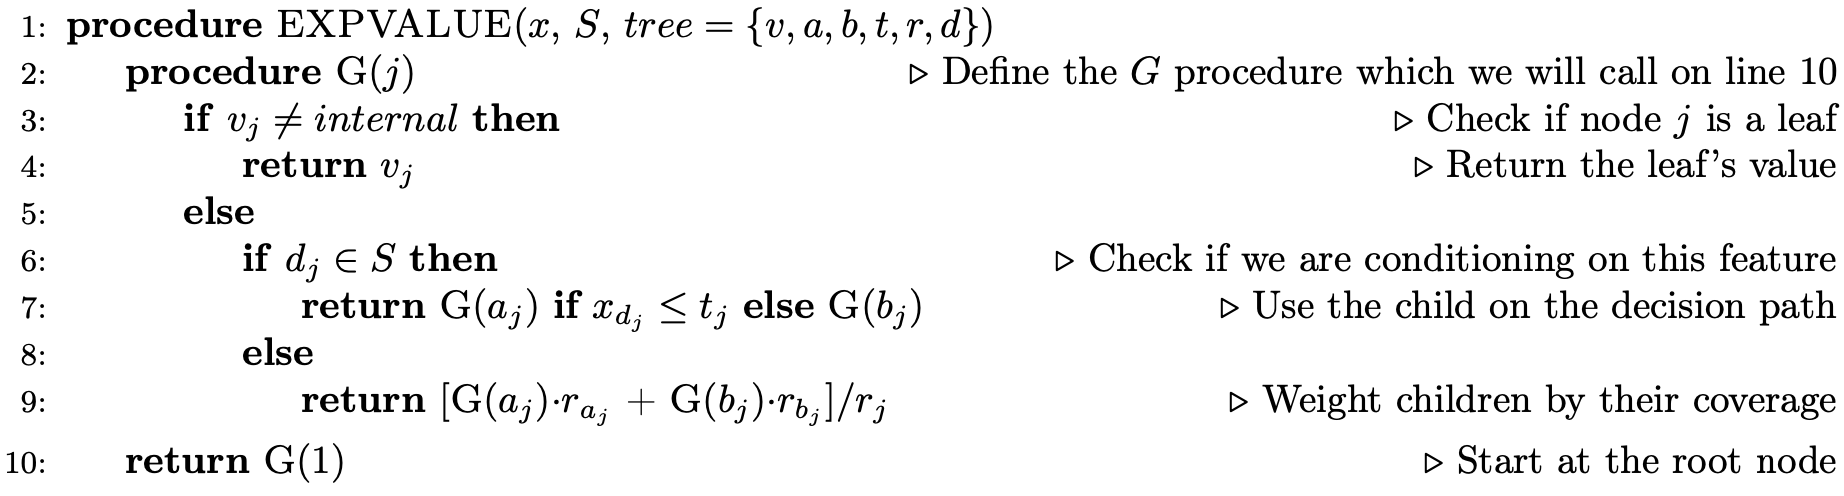
\includegraphics[width=0.95\textwidth]{images/treeSHAP_algo.png}
\end{figure}
\caption{}
\label{treeSHAP_algo}
\end{algorithm}
In the previous algorithm \textit{tree} contains the information of the tree:
\begin{itemize}
    \item '\textit{v}' is a vector of node values; 
    \item For internal nodes, we assign the value '\textit{internal}';
    \item The vectors '\textit{a}' and '\textit{b}' represent the left and right node indexes for each internal node;
    \item The vector '\textit{t}' contains the thresholds for each internal node, and d is a vector of indexes of the features used for splitting in internal nodes;
    \item The vector '\textit{r}' represents the cover of each node (i.e., how many data samples fall in that sub-tree).
\end{itemize}
This algorithm is actually a simpler and slower version of another more complex. The latter achieves same results but in polynomial time instead of exponential time and with just some main differences in the implementation.\\
The intuition of the polynomial time algorithm is to recursively keep track of what proportion of all possible subsets flow down into each of the leaves of the tree. This is similar to running \autoref{treeSHAP_algo} simultaneously for all $2^{M}$ subsets S in \autoref{eqn:estimation_formula}.\\

Also for Tree SHAP, we provide an example \textcolor{blue}{\href{https://colab.research.google.com/drive/1Q3TipsvwM6dQQtzT-WEOCvwS5UdvUwut?usp=sharing} {notebook}}, where we include a practical example and some of the most interesting new data visualization belonging to the implementation of Tree Shap in \texttt{TreeExplainer \href{https://github.com/slundberg/shap}{\textcolor{blue}{shap}}} python package.

\subsection{Deep SHAP (DeepLIFT + Shapley values)}
%https://towardsdatascience.com/pytorch-shap-explainable-convolutional-neural-networks-ece5f04c374f
%https://slundberg.github.io/shap/notebooks/deep_explainer/Front%20Page%20DeepExplainer%20MNIST%20Example.html
As mentioned before, model-dependant approximations like Deep SHAP promise to improve computational performance while extracting extra knowledge on the compositional nature of deep networks.
Deep SHAP incorporates another algorithm, DeepLIFT (Learning Important FeaTures), that also tries to interpret neural networks' "black box" nature, improving its flexibility and reliability. \\

DeepLIFT is a recursive prediction explanation method for deep learning presented in 2017 by A. Shrikumar et al.. It attributes to each input $x_{i}$ a value $C_{\Delta x_{i} \Delta t}$, called contribution scores, that represents the effect of that input being set to a reference value as opposed to its original value. This means that for DeepLIFT, the mapping $x = h_{x}(x^{'})$ converts binary values into the original inputs, where 1 indicates that an input takes its original value, and 0 indicates that it takes the reference value \cite{Interpreting-Model-Predictions}.
In other words, DeepLIFT aims to explain the difference in the output from some reference output in terms of the difference of the input from some reference input. If the output of a neuron for a given input has a difference $\Delta_{t}$ with its reference output, we can assign contribution scores to the differences of the activations of neurons in any intermediate layer with their reference state (i.e. $\Delta x_{i}$) such as following '\textit{summation-to-delta}' property \cite{DeepLIFT}:
\begin{equation}\label{eqn:summation-to-delta}
    \sum_{i=1}^{n}C_{\Delta x_{i} \Delta t} = \Delta_{t}
\end{equation}\\
Since DeepLIFT is an additive feature attribution method that satisfies local accuracy and missingness, we know that Shapley values represent the only attribution values that satisfy consistency. Therefore, adapting DeepLIFT to become a compositional approximation of SHAP values, leading to Deep SHAP was a simple consequence.

In short, Deep SHAP can efficiently compute SHAP values for the simple network components if they are linear functions, max pooling, or an activation function with just one input, this composition rule enables a fast approximation of values for the whole model. Deep SHAP avoids the need to heuristically choose ways to linearize components. Instead, it derives an effective linearization from the SHAP values computed for each component \cite{Interpreting-Model-Predictions}.\\

Finally for Deep SHAP, we prepared an example \textcolor{blue}{\href{https://colab.research.google.com/drive/1mkUgZO_04Tv5ojWPF8hSb6VROcfpbfTE?usp=sharing} {notebook}}, where we include a practical example and some of the most interesting new data visualization belonging to the implementation of Deep Shap in \texttt{DeepExplainer \href{https://github.com/slundberg/shap}{\textcolor{blue}{shap}}} python package.

